\chapter{Results and discussions}
\label{chp:resdisc}
\section{HLS output from LegUp}

\section{\label{sec:encprob}Encountered problems}
Throughout the work with LegUp, multiple problems that limits its usefulness towards \gls{asic}-applications has been encountered. The following section will describe some of the problems and their implication for the synthesis results described in section \ref{sec:synthres}, as well as for the continuation of the project.
\subsection{\label{subsec:memctrl}Memory controller}
In order to communicate between different modules instantiated in the top-module of the output Verilog from LegUp, a memory controller is declared and instantiated. All variables detected as global by LegUp, i.e. it is used by multiple modules or declared as a pointer and the points-to analysis fails to determine the exact array for the pointer at compile-time, is stored in a ram module inside this memory controller. This approach is well intended for the hybrid flow supported by LegUp, where a soft-processor works in cooperation with one or more functions implemented as hardware accelerators in an \gls{fpga}, meaning that data needs to be transferred between the software and hardware portion of the system. For an \gls{asic}, pure-\gls{hw} implementation however, this approach creates a lot of extra overhead and basically does not provide any additional functionality to the circuitry. In the pure-\gls{hw} flow in LegUp, all the functionality described under the main-function in the input C-code will be translated into a single \gls{fsm}. The main function is further the only module instantiated under the top-module in the produced Verilog, besides the memory controller. The use of the memory controller is in itself not an issue as LegUp handles all memory access automatically, but this will come at the expense of both decreased speed and increased area usage. It will also cause some problems related to input and output, as described in subsection \ref{subsec:inoutprobs}.
\subsection{\label{subsec:inoutprobs}Inputs and outputs}
When designing a hardware module, its task can vary almost infinitely. However, most modules takes some input data together with some control signals, does something with the data and outputs some kind of response. This makes input and outputs, and the ability to configure them properly, extremely important in most module design. In the documentation on the LegUp web-page, the developers claim that each function declared in C is translated into a corresponding module in Verilog. However, \gls{hls}-output shows that in the pure-\gls{hw} flow, the only generated module is the one containing the main-function, as describe in subsection \ref{subsec:memctrl}. As LegUp uses a standard C compiler front-end for \gls{llvm} to compile the C-code into \gls{llvm}-\gls{ir}, we need to follow the \gls{ansi}-C specification when writing our C-code. In a standard programming case, the main() function has a special purpose, specifically, the run-time environment calls this function to start execution of the program. The return value of the main function is defined to be an int, who's purpose is to return program execution status to the invoker process. The main function is also defined to handle arguments input from command-line, through the input arguments \textit{int argc} and \textit{char *argv[]}, where \textit{argc} is the number of command-line arguments, and \textit{*argv} is an array of pointers to the given arguments. The implications of this is that if we want inputs and outputs to or from the module we design in out C-code, we are limited to the arguments allowed through the defined main-function in the \gls{ansi}-C specifications. Further, this problem increases when we realize that any inputs or outputs except one int for each has to be a pointer, which entails it has to go through the above described memory controller. This causes a lot of overhead, as most input- and output-data has to be written to and read from memory, creating the need for a dedicated custom module for handling I/O. Adding the flag \textit{-ffreestanding} to the makefile fixes this problem by not issuing the error. Return values still need to be single variable, pointer or struct (struct not supported without altsyncram)
\subsection{Bus widths}
When designing digital hardware circuits, you often want (and in some cases need) to use bit-vectors of a given size. Since \gls{ansi}-C does not have built-in support for data-types of other sizes than 8, 16, 32 and 64 bits, this causes problems when doing \gls{hls}. LegUp does however have a class, \textit{MinimizeBitwidth.cpp}, which calculate the minimum needed bits in a signal an limits the width to this size, but this does only work for internal signals, where all values assigned to the variable is known at compile-time. If the signal shall be an input or output, the maximum value of the signal is not known, and it can therefore not be limited. Having too wide signals will increase the occupied area since all components must support the extra bits. A simple example is shown in figure \ref{fig:andgate34}, where we can easily see that the addition of one extra bit to the input signal adds one extra 2-input AND gate to the circuit.
\begin{figure}[hbpt]
\centering
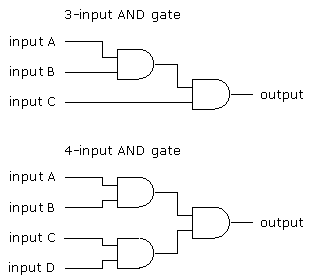
\includegraphics[width=0.6\textwidth]{../figs/AndGate34Bit.png}
\caption{\label{fig:andgate34}3-bit input versus 4-bit input AND-gate}
\end{figure}
Technically this is a limitation inherited from the lack of logical data-types in C, but this problem needs to be addressed if LegUp shall be used as an architectural exploration framework.
\subsection{\label{subsec:parameterprobs}Parameters}
The lack of support for transferring parameters from the C code into the generated Verilog makes it harder to instantiate modules based on widths or depths of different parameters. Often this is desirable in order to reuse the modules for a variety of given parameter values.
\section{\label{sec:synthres}Synthesis results}
Due to the above mentioned problems, some manual alteration of the generated Verilog had to be made in order for the results from LegUp to be comparable to the results from the native Verilog.